% Document Class
\documentclass[12pt,a4paper]{article}

% Packages
\usepackage[utf8]{inputenc}
\usepackage[T1]{fontenc}
\usepackage{mathptmx} % Times New Roman
\usepackage{courier}  % Courier for monospace
\usepackage{helvet}   % Helvetica for sans-serif
\usepackage{amsmath}
\usepackage[english,indonesian]{babel}
\usepackage{geometry}
\usepackage{setspace}
\usepackage{titlesec}
\usepackage{graphicx}
\usepackage{hyperref}
\usepackage{booktabs}
\usepackage{array}
\usepackage[format=hang,font=footnotesize,labelfont=bf]{caption}
\usepackage{enumitem}
\usepackage{parskip}
\usepackage{fancyhdr}
\usepackage{tocloft}
\usepackage{tabularx}
\usepackage{longtable}
\usepackage{ragged2e}
\usepackage{float}
\usepackage{listings}
\usepackage{xurl}
\usepackage{xcolor}

% Configuration for listings (Python)
\definecolor{codegreen}{rgb}{0,0.6,0}
\definecolor{codegray}{rgb}{0.5,0.5,0.5}
\definecolor{codepurple}{rgb}{0.58,0,0.82}
\definecolor{backcolour}{rgb}{0.95,0.95,0.92}

\lstset{
    language=Python,
    backgroundcolor=\color{backcolour},   
    commentstyle=\color{codegreen},
    keywordstyle=\color{magenta},
    numberstyle=\tiny\color{codegray},
    stringstyle=\color{codepurple},
    basicstyle=\ttfamily\scriptsize,
    breakatwhitespace=false,         
    breaklines=true,                 
    captionpos=b,                    
    keepspaces=true,                 
    numbers=left,                    
    numbersep=5pt,                  
    showspaces=false,                
    showstringspaces=false,
    showtabs=false,                  
    tabsize=2
}

% Page Setup
\geometry{
    top=3cm,
    bottom=3cm,
    left=4cm,
    right=3cm
}

% Title Formatting
\titleformat{\section}[display]
    {\normalfont\fontsize{14}{17}\bfseries\centering}
    {PRAKTIKUM \thesection}{0pt}{}
    
\titleformat{\subsection}
    {\normalfont\fontsize{12}{14}\bfseries}{\thesubsection}{1em}{}

% Spacing
\onehalfspacing

% Header/Footer
\pagestyle{fancy}
\fancyhf{}
\renewcommand{\headrulewidth}{0pt}

% Gaya halaman untuk Front Matter (nomor di tengah)
\fancypagestyle{frontmatter}{
    \fancyhf{}
    \fancyfoot[C]{\thepage}
}

% Gaya halaman untuk Main Matter (nomor di kanan)
\fancypagestyle{mainmatter}{
    \fancyhf{}
    \fancyfoot[R]{\thepage}
}

% Redefine plain style (used by \section) to match mainmatter
\fancypagestyle{plain}{
    \fancyhf{}
    \fancyfoot[R]{\thepage}
}

% Data Identitas
\newcommand{\txtTitle}{LAPORAN PRAKTIKUM SRATEGI ALGORITMA}
\newcommand{\txtSubtitle}{MATA KULIAH SRATEGI ALGORITMA}
\newcommand{\txtNama}{RADITYA RIZKI RAHARJA}
\newcommand{\txtNIM}{714240041}
\newcommand{\txtKelas}{2A}
\newcommand{\txtDosen}{RONI HABIBI, S.KOM., M.T., SFPC}
\newcommand{\txtYear}{2026}

% Redefine maketitle
\makeatletter
\renewcommand{\maketitle}{
    \begin{titlepage}
        \centering
        \setstretch{1.2}
        
        \vspace*{1cm}
        
        % Judul Utama
        {\fontsize{16}{20}\selectfont\textbf{\txtTitle}\par}
        \vspace{0.5cm}
        {\fontsize{14}{18}\selectfont\textbf{\txtSubtitle}\par}
        
        \vspace{1.5cm}
        
        % Logo
        \IfFileExists{logo.png}{
            \includegraphics[width=0.5\textwidth]{logo.png}
        }{
            \vspace{2cm}
            {\fontsize{20}{24}\bfseries LOGO ULBI\par}
            \vspace{2cm}
        }
        
        \vspace{1.5cm}
        
        % Disusun Oleh
        {\fontsize{12}{14}\selectfont\textbf{DISUSUN OLEH:}\par}
        \vspace{0.5cm}
        \begin{tabular}{ll}
            {\fontsize{12}{14}\selectfont \textbf{NAMA}} & {\fontsize{12}{14}\selectfont \textbf{: \txtNama}} \\
            {\fontsize{12}{14}\selectfont \textbf{NIM}}  & {\fontsize{12}{14}\selectfont \textbf{: \txtNIM}} \\
            {\fontsize{12}{14}\selectfont \textbf{KELAS}} & {\fontsize{12}{14}\selectfont \textbf{: \txtKelas}}
        \end{tabular}
        
        \vspace{1.5cm}
        
        % Dosen Pengampu
        {\fontsize{12}{14}\selectfont\textbf{DOSEN PENGAMPU:}\par}
        \vspace{0.5cm}
        {\fontsize{12}{14}\selectfont \textbf{\txtDosen}\par}
        
        \vfill
        
        % Footer
        {\fontsize{14}{17}\selectfont
        \textbf{PROGRAM STUDI DIV TEKNIK INFORMATIKA}\par
        \textbf{UNIVERSITAS LOGISTIK \& BISNIS INTERNASIONAL}\par
        \textbf{BANDUNG}\par
        \textbf{\txtYear}\par}
        
        \vspace*{1cm}
    \end{titlepage}
    \newpage
}
\makeatother

% Bibliography Setup
\usepackage[
    backend=biber,
    style=ieee,
    sorting=none,
    maxbibnames=99,
    dashed=false,
    url=false,
    doi=true,
]{biblatex}
\addbibresource{references.bib}

% TOC, LOT, LOF Centering
\renewcommand{\cfttoctitlefont}{\hfill\fontsize{14}{17}\bfseries}
\renewcommand{\cftaftertoctitle}{\hfill}
\renewcommand{\cftlottitlefont}{\hfill\fontsize{14}{17}\bfseries}
\renewcommand{\cftafterlottitle}{\hfill}
\renewcommand{\cftloftitlefont}{\hfill\fontsize{14}{17}\bfseries}
\renewcommand{\cftafterloftitle}{\hfill}

% Beginning of Document
\begin{document}

% Force TOC title to be uppercase (fix for babel override)
\renewcommand{\contentsname}{DAFTAR ISI}
\renewcommand{\listtablename}{DAFTAR TABEL}
\renewcommand{\listfigurename}{DAFTAR GAMBAR}

\rmfamily
\maketitle

% Front Matter
\pagenumbering{roman}
\pagestyle{frontmatter}

% Override plain style for frontmatter to keep it centered
\fancypagestyle{plain}{
    \fancyhf{}
    \fancyfoot[C]{\thepage}
}

\phantomsection
\addcontentsline{toc}{section}{DAFTAR ISI}
\tableofcontents
\clearpage

\phantomsection
\addcontentsline{toc}{section}{DAFTAR TABEL}
\listoftables
\clearpage

\phantomsection
\addcontentsline{toc}{section}{DAFTAR GAMBAR}
\listoffigures
\clearpage

% Main Content
\pagenumbering{arabic}
\setcounter{page}{1}
\pagestyle{mainmatter}

% Override plain style for mainmatter to keep it on the right
\fancypagestyle{plain}{
    \fancyhf{}
    \fancyfoot[R]{\thepage}
}

% Praktikum 1
\section{KOMPLEKSITAS ALGORITMA}
\subsection{Definisi}
Konten definisi praktikum 1.
\subsection*{Pertanyaan 1: Apa alat ukur sebuah algoritma dikatakan efisien menjadi solusi suatu permasalahan?}

\textbf{Jawaban:} Alat ukur efisiensi algoritma ada dua: Kompleksitas Waktu T(n) yang mengukur jumlah operasi komputasi sebagai fungsi ukuran masukan n, dan Kompleksitas Ruang S(n) yang mengukur kebutuhan memori. Keduanya bersifat abstrak dan independen dari perangkat keras maupun compiler sehingga dapat digunakan sebagai acuan universal dalam membandingkan algoritma.

\subsection*{Pertanyaan 2: Mengapa kita perlu algoritma yang efisien?}

\textbf{Jawaban:} Algoritma yang efisien diperlukan karena:
\begin{enumerate}
    \item Selisih kompleksitas sangat terasa pada data besar. Untuk $n = 1.000.000$, algoritma $O(n)$ butuh $10^6$ operasi sedangkan $O(n^2)$ butuh $10^{12}$ operasi.
    \item Menghemat sumber daya komputasi berupa waktu proses, memori, dan energi.
    \item Memungkinkan sistem yang skalabel karena performa tetap baik meskipun data bertambah.
\end{enumerate}

\subsection{Langkah Praktikum: Selection Sort}

\subsubsection*{Flowchart}
\begin{figure}[H]
    \centering
    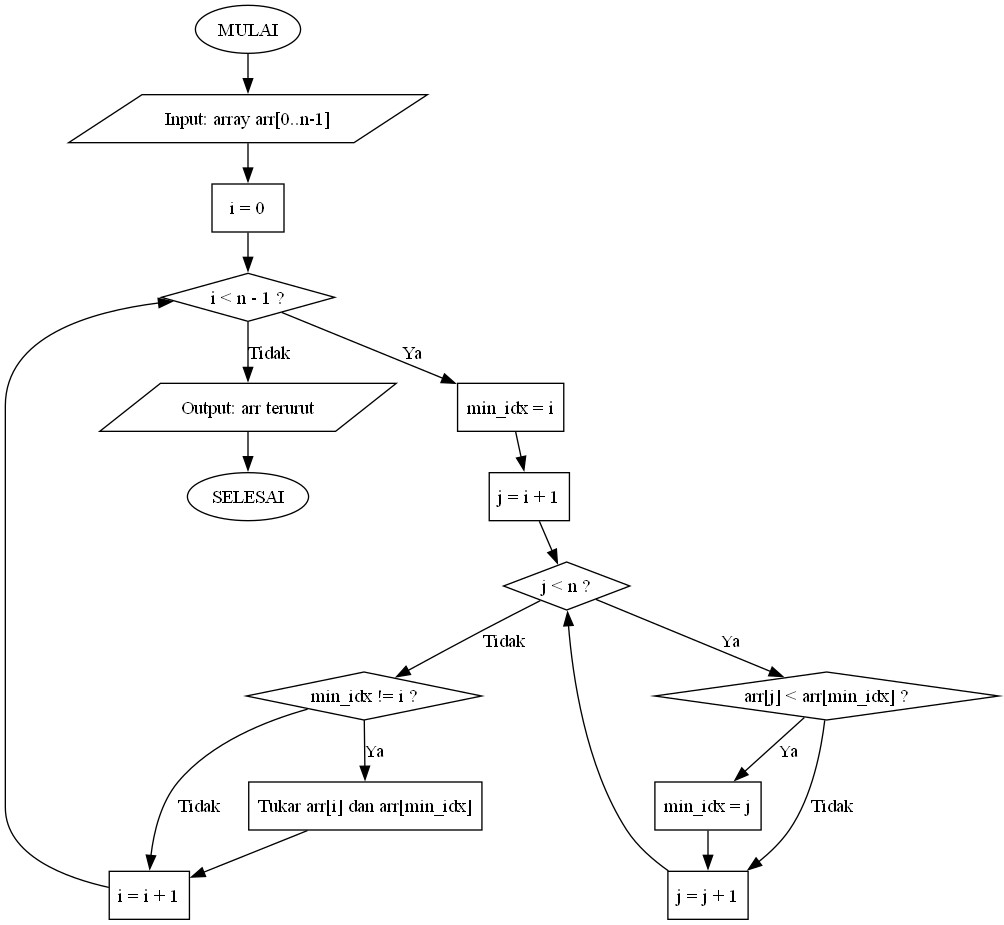
\includegraphics[width=0.65\textwidth]{figures/praktikum1/flowchart_selection_sort.png}
    \caption{Flowchart Algoritma Selection Sort}
\end{figure}

\subsubsection*{Source Code Python}
\begin{lstlisting}[basicstyle=\ttfamily\scriptsize, frame=single, backgroundcolor=\color{white}, numbers=none, keywordstyle=\color{black}, commentstyle=\color{black}, stringstyle=\color{black}, breaklines=true]
def selection_sort(arr):
    """
    Mengurutkan array dengan algoritma Selection Sort.
    Setiap pass mencari elemen terkecil dari sisa array
    lalu menukarnya ke posisi yang tepat.
    """
    n = len(arr)
    total_comparisons = 0
    total_swaps = 0
    print(f"Array awal : {arr}")
    print("-" * 55)

    for i in range(n - 1):
        # Asumsikan elemen terkecil ada di posisi i
        min_idx = i
        pass_comparisons = 0
        pass_swaps = 0

        # Cari elemen terkecil dari i+1 hingga akhir array
        for j in range(i + 1, n):
            pass_comparisons += 1
            if arr[j] < arr[min_idx]:
                min_idx = j

        # Tukar elemen terkecil ke posisi i (jika berbeda)
        if min_idx != i:
            arr[i], arr[min_idx] = arr[min_idx], arr[i]
            pass_swaps += 1

        total_comparisons += pass_comparisons
        total_swaps += pass_swaps

        print(f"Pass {i + 1:2d} | Array: {arr} | "
              f"Perbandingan: {pass_comparisons:2d} | "
              f"Pertukaran: {pass_swaps}")
        print("-" * 55)

    print(f"Array akhir : {arr}")
    print(f"Total perbandingan : {total_comparisons}")
    print(f"Total pertukaran   : {total_swaps}")
    return arr
\end{lstlisting}

\subsubsection*{Analisis}
\textbf{Jawaban 1: Jumlah operasi perbandingan untuk setiap pass ke-i}\\
Pada pass ke-i (i dari 0 sampai n-2), algoritma mencari elemen minimum dari posisi i+1 hingga n-1. Jumlah perbandingan pada setiap pass disajikan pada Tabel \ref{tab:perbandingan_selection}:

\begin{table}[H]
    \centering
    \caption{Operasi Perbandingan Per Pass Selection Sort}
    \label{tab:perbandingan_selection}
    \begin{tabular}{ccc}
    \toprule
    \textbf{Pass ke-i} & \textbf{Rentang Pencarian} & \textbf{Perbandingan} \\ \midrule
    0 & A[1] hingga A[4] & 4 \\
    1 & A[2] hingga A[4] & 3 \\
    2 & A[3] hingga A[4] & 2 \\
    3 & A[4] hingga A[4] & 1 \\ \bottomrule
    \end{tabular}
\end{table}

\textbf{Jawaban 2: Jumlah operasi pertukaran elemen}\\
Setiap pass melakukan paling banyak 1 kali pertukaran, hanya apabila elemen minimum (min\_idx) bukan berada di posisi i. Pertukaran minimum 0 kali (array sudah terurut) dan maksimum n-1 kali. Pada Kasus Uji 1 dengan n=5, total pertukaran = 3 dari 4 pass.

\textbf{Jawaban 3: Derivasi kompleksitas waktu}\\
Total perbandingan dijumlahkan dari seluruh pass:
\[ T(n) = (n-1) + (n-2) + ... + 1 = n(n-1) / 2 \]
Untuk n=5: T(5) = 5 $\times$ 4 / 2 = 10, sesuai output program. Suku dominan adalah $n^2$, sehingga kompleksitas waktu Selection Sort adalah $O(n^2)$.


\subsection{Post Test: Insertion Sort}

\subsubsection*{Flowchart}
\begin{figure}[H]
    \centering
    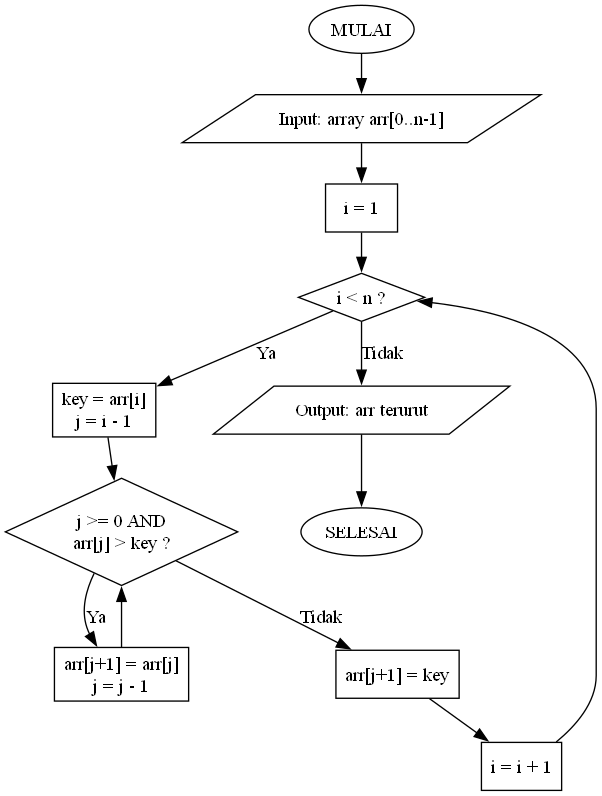
\includegraphics[width=0.65\textwidth]{figures/praktikum1/flowchart_insertion_sort.png}
    \caption{Flowchart Algoritma Insertion Sort}
\end{figure}

\subsubsection*{Source Code Python}
\begin{lstlisting}[basicstyle=\ttfamily\scriptsize, frame=single, backgroundcolor=\color{white}, numbers=none, keywordstyle=\color{black}, commentstyle=\color{black}, stringstyle=\color{black}, breaklines=true]
def insertion_sort(arr):
    """
    Mengurutkan array dengan algoritma Insertion Sort.
    Setiap elemen disisipkan ke posisi yang tepat
    di dalam bagian array yang sudah terurut.
    """
    n = len(arr)
    total_comparisons = 0
    total_shifts = 0
    print(f"Array awal : {arr}")
    print("-" * 60)

    for i in range(1, n):
        key = arr[i]
        j = i - 1
        pass_comparisons = 0
        pass_shifts = 0

        # Geser elemen yang lebih besar dari key ke kanan
        while j >= 0 and arr[j] > key:
            arr[j + 1] = arr[j]
            j -= 1
            pass_comparisons += 1
            pass_shifts += 1

        # Hitung perbandingan terakhir (kondisi berhenti)
        if j >= 0:
            pass_comparisons += 1

        # Sisipkan key ke posisi yang tepat
        arr[j + 1] = key
        total_comparisons += pass_comparisons
        total_shifts += pass_shifts

        print(f"Pass {i:2d} | key={key:3d} | Array: {arr} | "
              f"Perbandingan: {pass_comparisons} | "
              f"Pergeseran: {pass_shifts}")
        print("-" * 60)

    print(f"Array akhir        : {arr}")
    print(f"Total perbandingan : {total_comparisons}")
    print(f"Total pergeseran   : {total_shifts}")
    return arr
\end{lstlisting}

\subsubsection*{Analisis}
\textbf{Jawaban 1: Kompleksitas waktu Insertion Sort}
\begin{itemize}
    \item \textbf{Best Case O(n):} Array sudah terurut. Setiap elemen hanya dibandingkan sekali, tidak ada pergeseran. T(n) = n-1.
    \item \textbf{Worst Case O(n$^2$):} Array terurut terbalik. Elemen ke-i harus digeser i kali. T(n) = 1+2+...+(n-1) = n(n-1)/2.
    \item \textbf{Average Case O(n$^2$):} Rata-rata elemen ke-i melakukan i/2 perbandingan. T(n) $\approx$ n(n-1)/4.
\end{itemize}

\textbf{Jawaban 2: Perbandingan Selection Sort vs Insertion Sort}
Tabel \ref{tab:komparasi_sort} merangkum perbedaan karakteristik antara kedua algoritma pengurutan tersebut:

\begin{table}[H]
    \centering
    \caption{Perbandingan Selection Sort dan Insertion Sort}
    \label{tab:komparasi_sort}
    \begin{tabular}{lll}
    \toprule
    \textbf{Aspek} & \textbf{Insertion Sort} & \textbf{Selection Sort} \\ \midrule
    Best Case & O(n) --- adaptif & O(n$^2$) --- tidak adaptif \\
    Worst Case & O(n$^2$) & O(n$^2$) \\
    Average Case & O(n$^2$) & O(n$^2$) \\
    Pertukaran/Geser & Banyak (pergeseran) & Sedikit (maks. n-1) \\
    Stabilitas & Stabil & Tidak Stabil \\
    Adaptivitas & Adaptif & Tidak Adaptif \\ \bottomrule
    \end{tabular}
\end{table}

\textbf{Kesimpulan:} Insertion Sort lebih mangkus pada data yang hampir terurut karena bersifat adaptif dengan best case O(n). Selection Sort lebih unggul dalam minimasi pertukaran (maks. n-1 swap), cocok ketika operasi swap memiliki biaya mahal. Pada data acak berukuran besar keduanya setara di $O(n^2)$.

\subsection{Implementasi Nyata}
Selection Sort dan Insertion Sort banyak diimplementasikan pada sistem dengan dataset kecil, seperti sistem pengolahan nilai akademik, antrian transaksi sederhana, atau pengurutan log pada embedded system. Dua jurnal berikut mendukung relevansi penggunaan kedua algoritma ini dalam praktik.

\vspace{1em}
\textbf{[1] Penulis:} Karunanidhi, G. (2025)

\textbf{Judul:} "A Systematic Analysis on Performance and Computational Complexity of Sorting Algorithms"

\textbf{Publikasi:} Discover Computing, Vol. 28, No. 1, Hal. 250. Springer Nature. DOI: 10.1007/s10791-025-09724-w

\textbf{Intisari:} Review sistematis terhadap 12 teknik sorting klasik menggunakan analisis empiris pada MATLAB dengan ukuran data 100 hingga 100.000 elemen. Hasil menunjukkan bahwa selection sort mengalami penurunan performa signifikan pada data besar karena kompleksitas $O(n^2)$ yang konsisten di semua kasus. Sebaliknya, insertion sort terbukti lebih efisien untuk data berukuran kecil berkat sifat adaptifnya.

\textbf{Link:} \url{https://link.springer.com/article/10.1007/s10791-025-09724-w}

\vspace{1.5em}
\textbf{[2] Penulis:} Halili, F. dan Dika, E. (2021)

\textbf{Judul:} "Results of Comparison Between Different Sorting Algorithms"

\textbf{Publikasi:} IBU International Journal of Technical and Natural Sciences, Vol. 2, Hal. 39-52. International Balkan University Press.

\textbf{Intisari:} Studi komparatif lima algoritma pengurutan berdasarkan waktu eksekusi menggunakan C++. Hasil empiris menunjukkan bahwa Insertion Sort merupakan pilihan yang baik untuk dataset berukuran kecil hingga beberapa ribu elemen karena sifat adaptif (best case O(n)) dan kemudahan implementasinya. Insertion Sort tidak disarankan untuk list dengan lebih dari beberapa ribu elemen karena kompleksitas kuadratiknya.

\textbf{Link:} \url{https://ijtns.ibupress.com/uploads/pdf/22.pdf}

\vspace{1.5em}
\textbf{Kelebihan di konteks dataset kecil:}
\begin{itemize}
    \item Implementasi sederhana dan mudah dipelihara.
    \item Tidak memerlukan memori tambahan (in-place).
    \item Insertion Sort efisien untuk data yang ditambahkan secara bertahap (inkremental).
\end{itemize}

\textbf{Kekurangan di konteks dataset kecil:}
\begin{itemize}
    \item Tidak cocok untuk $n > 10.000$ karena kompleksitas $O(n^2)$ menjadi bottleneck.
    \item Untuk kebutuhan skala besar, disarankan beralih ke Merge Sort atau Quick Sort dengan kompleksitas $O(n \log n)$.
\end{itemize}

\clearpage

% Praktikum 2
\section{ALGORITMA BRUTE FORCE}
\subsection{Definisi}
Konten definisi praktikum 2.
\subsection*{Pertanyaan 1: Jelaskan apa ciri khas dari penyelesaian persoalan dengan algoritma Brute Force!}

\textbf{Jawaban:} Ciri khas Brute Force adalah penyelesaian masalah secara langsung, sederhana, dan jelas (straightforward/obvious way) tanpa memanfaatkan struktur atau sifat khusus dari masalah. Setiap kemungkinan diperiksa satu per satu secara menyeluruh. Pendekatan ini menjamin solusi yang benar namun umumnya menghasilkan kompleksitas yang tinggi karena tidak ada optimasi.

\subsection*{Pertanyaan 2: Jelaskan ciri khas algoritma Brute Force pada contoh berikut:}

\textbf{a. Algoritma Perpangkatan:} Brute Force terlihat dari cara menghitung $a^n$ dengan mengalikan $a$ sebanyak $n$ kali secara berulang (hasil = hasil * a), tanpa memanfaatkan teknik seperti fast exponentiation. Kompleksitas O(n).

\textbf{b. Algoritma Pencarian Elemen Terbesar:} Brute Force terlihat dari pembandingan setiap elemen A[k] dengan nilai maks satu per satu dari awal hingga akhir array. Tidak ada strategi pemangkasan. Kompleksitas O(n).

\textbf{c. Algoritma Perkalian Dua Matriks:} Brute Force terlihat dari tiga perulangan bersarang (i, j, k) yang menghitung setiap elemen C[i][j] satu per satu tanpa optimasi. Kompleksitas O($n^3$).

\textbf{d. Algoritma Uji Bilangan Prima:} Brute Force terlihat dari pembagian x dengan setiap bilangan dari 2 hingga sqrt(x) secara berurutan. Tidak ada penggunaan sifat bilangan prima untuk mempercepat. Kompleksitas O($\sqrt{n}$).
\subsection{Analisis Praktikum}
Analisis langkah dan post test praktikum 2.
\subsection{Implementasi Nyata}
Algoritma Brute Force seperti pencarian elemen terbesar dan uji bilangan prima digunakan secara nyata dalam berbagai bidang, mulai dari kriptografi hingga sistem keamanan jaringan. Jurnal berikut mendukung relevansinya.

\vspace{1em}
\textbf{[1] Penulis:} Baur, K. et al. (2023)\\
\textbf{Judul:} "Comparing and Reviewing Modern Primality Tests"\\
\textbf{Publikasi:} ResearchGate, 2023. Tersedia di: \url{https://www.researchgate.net/publication/369685477}\\
\textbf{Intisari:} Makalah ini membandingkan berbagai algoritma uji bilangan prima mulai dari Brute Force trial division (O($\sqrt{n}$)) hingga algoritma modern seperti Miller-Rabin dan AKS. Brute Force digunakan sebagai baseline referensi karena kesederhanaan dan ketepatannya. Hasilnya menunjukkan bahwa Brute Force masih relevan untuk bilangan kecil, namun tidak skalabel untuk bilangan kriptografis berukuran besar (ratusan digit).\\
\textbf{Link:} \url{https://www.researchgate.net/publication/369685477_Comparing_and_Reviewing_Modern_Primality_Tests}

\vspace{1em}
\textbf{Kelebihan dalam konteks nyata:}
\begin{itemize}
    \item Implementasi sederhana dan mudah diverifikasi kebenarannya.
    \item Cocok sebagai baseline perbandingan sebelum menggunakan algoritma yang lebih kompleks.
    \item Uji bilangan prima O($\sqrt{n}$) sudah cukup efisien untuk kebutuhan pembuatan kunci pada sistem kriptografi skala kecil.
\end{itemize}

\textbf{Kekurangan dalam konteks nyata:}
\begin{itemize}
    \item Tidak skalabel: untuk bilangan prima kriptografis (ratusan digit), kompleksitas O($\sqrt{n}$) masih terlalu lambat dan perlu diganti algoritma probabilistik seperti Miller-Rabin.
    \item Pencarian elemen terbesar O(n) memang sudah optimal untuk kasus linear, namun tidak berlaku jika data terstruktur (misal sudah terurut) yang memungkinkan pencarian lebih cepat.
\end{itemize}
\clearpage

% Praktikum 3
\section{ALGORITMA GREEDY}
\subsection{Definisi}
Konten definisi praktikum 3.
\subsection{Pre Test}
Jawaban pre test praktikum 3.
\subsection{Langkah Praktikum: Coin Exchange}

\subsubsection*{Flowchart}
\begin{figure}[H]
    \centering
    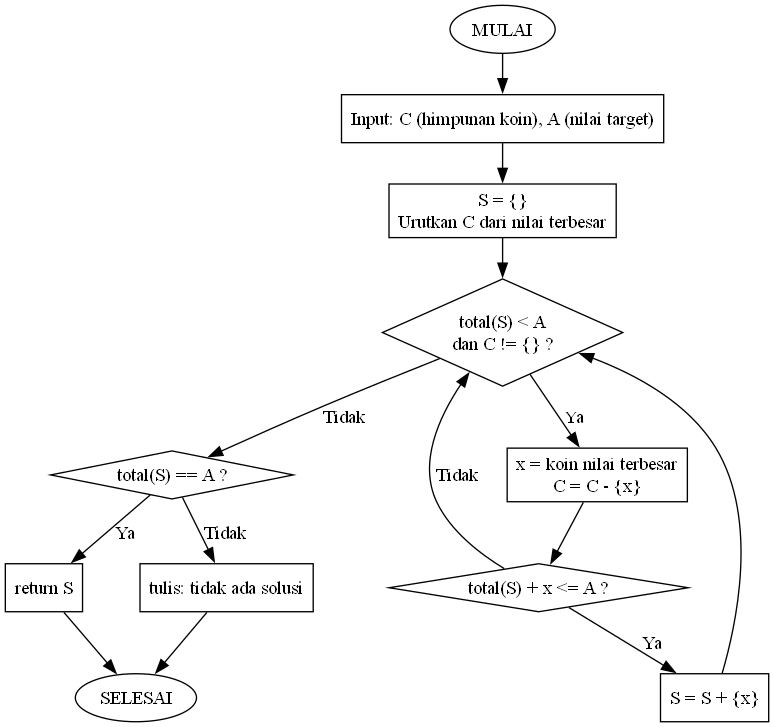
\includegraphics[width=0.55\textwidth]{figures/praktikum3/flowchart_coin_exchange.png}
    \caption{Flowchart Algoritma Coin Exchange}
\end{figure}

\subsubsection*{Source Code Python}
\begin{lstlisting}[basicstyle=\ttfamily\scriptsize, frame=single, backgroundcolor=\color{white}, numbers=none, keywordstyle=\color{black}, commentstyle=\color{black}, stringstyle=\color{black}, breaklines=true]
def coin_exchange(coins, amount):
    # urutkan koin dari nilai terbesar ke terkecil (strategi greedy)
    coins_sorted = sorted(coins, reverse=True)
    result = []
    remaining = amount

    for coin in coins_sorted:
        # ambil koin sebanyak mungkin selama tidak melebihi sisa
        while remaining >= coin:
            result.append(coin)
            remaining -= coin

    if remaining == 0:
        return result
    else:
        return None  # tidak ada solusi
\end{lstlisting}

\subsubsection*{Analisis Output}
Program diuji dengan koin standar [1000, 500, 200, 100, 50, 25, 10, 5, 1] dan nilai target 2750:

\begin{table}[H]
    \centering
    \caption{Proses Penukaran Koin dengan Pendekatan Greedy}
    \begin{tabular}{lll}
    \toprule
    \textbf{Langkah} & \textbf{Koin Dipilih} & \textbf{Sisa Nilai} \\ \midrule
    1 & 1000 & 1750 \\
    2 & 1000 & 750 \\
    3 & 500 & 250 \\
    4 & 200 & 50 \\
    5 & 50 & 0 \\ \bottomrule
    \end{tabular}
\end{table}

Hasil: koin yang digunakan = [1000, 1000, 500, 200, 50], total 5 koin. Algoritma greedy berhasil menemukan solusi minimal karena sistem koin Rupiah bersifat kanonik, artinya pilihan koin terbesar di setiap langkah selalu mengarah ke solusi dengan jumlah koin minimum.

\subsection{Post Test}

\subsubsection*{Source Code Python}
\begin{lstlisting}[basicstyle=\ttfamily\scriptsize, frame=single, backgroundcolor=\color{white}, numbers=none, keywordstyle=\color{black}, commentstyle=\color{black}, stringstyle=\color{black}, breaklines=true]
def analisis_kasus(coins, amount, label=""):
    print(f"\n{'='*50}")
    if label:
        print(f" {label}")
    print(f"{'='*50}")
    print(f"Nilai ditukar : {amount}")
    print(f"Koin tersedia : {sorted(coins, reverse=True)}")

    hasil = coin_exchange(coins, amount)

    if hasil:
        rekap = Counter(hasil)
        print(f"Solusi        : {dict(rekap)}")
        print(f"Jumlah koin   : {len(hasil)}")
    else:
        print("Tidak ada solusi (greedy gagal).")

    return hasil

def hitung_kompleksitas(coins, amount):
    # hitung iterasi aktual untuk analisis kompleksitas
    coins_sorted = sorted(coins, reverse=True)
    n = len(coins_sorted)
    iterasi = 0
    remaining = amount

    for coin in coins_sorted:
        while remaining >= coin:
            remaining -= coin
            iterasi += 1

    print(f"\nAnalisis Kompleksitas (amount={amount}, n={n} jenis koin):")
    print(f"Jumlah iterasi while : {iterasi}")
    print(f"Jumlah iterasi for   : {n}")
    print(f"T(n) = O(n + amount/koin_terkecil) -> praktis O(n) untuk denominasi wajar")

if __name__ == "__main__":
    koin_std = [1000, 500, 200, 100, 50, 25, 10, 5, 1]

    # kasus 1: solusi optimal
    analisis_kasus(koin_std, 2750, "Kasus 1: Solusi Normal")

    # kasus 2: jumlah besar
    analisis_kasus(koin_std, 9875, "Kasus 2: Jumlah Besar")

    # kasus 3: greedy tidak optimal (denominasi tidak kanonik)
    koin_non_kanonik = [10, 6, 1]
    analisis_kasus(koin_non_kanonik, 12, "Kasus 3: Greedy Tidak Optimal (koin [10,6,1], target 12)")
    print("  Solusi greedy: 10+1+1 = 3 koin")
    print("  Solusi optimal: 6+6   = 2 koin")

    # analisis kompleksitas
    hitung_kompleksitas(koin_std, 2750)
\end{lstlisting}

\textbf{Jawaban 1: Implementasi, output, dan analisis kasus}\\
Program diuji pada tiga kasus:
\begin{itemize}
    \item \textbf{Kasus 1 (nilai 2750, koin kanonik):} Solusi = \{1000:2, 500:1, 200:1, 50:1\}, total 5 koin. Greedy optimal.
    \item \textbf{Kasus 2 (nilai 9875, koin kanonik):} Solusi = \{1000:9, 500:1, 200:1, 100:1, 50:1, 25:1\}, total 14 koin. Greedy optimal.
    \item \textbf{Kasus 3 (nilai 12, koin [10,6,1] non-kanonik):} Solusi greedy = \{10:1, 1:2\} = 3 koin. Solusi optimal = \{6:2\} = 2 koin. Greedy tidak optimal karena sistem koin tidak kanonik.
\end{itemize}

Kasus 3 membuktikan bahwa algoritma Greedy tidak menjamin solusi optimal secara universal. Untuk sistem koin non-kanonik, diperlukan pendekatan Dynamic Programming.

\textbf{Jawaban 2: Kompleksitas waktu}\\
Analisis kompleksitas dilakukan berdasarkan dua komponen utama:
\begin{itemize}
    \item \textbf{Loop for iterasi jenis koin:} dilakukan sebanyak n kali (n = jumlah jenis koin). Kompleksitas O(n).
    \item \textbf{Loop while pengambilan koin:} untuk setiap jenis koin, jumlah pengambilan bergantung pada nilai koin dan sisa amount. Dalam kasus terburuk total iterasi while = floor(A / koin\_terkecil).
\end{itemize}

Sehingga total kompleksitas:
\[ T(n) = O(n + A / d\_min) \]

dengan n = jumlah jenis koin dan d\_min = nilai koin terkecil. Untuk sistem mata uang praktis (d\_min = 1), kasus terburuk adalah T(n) = O(A). Namun secara praktis karena koin terbesar mendominasi pengambilan, jumlah iterasi while jauh lebih kecil dari A sehingga kompleksitas efektif mendekati O(n).

\begin{table}[H]
    \centering
    \caption{Kompleksitas Waktu Algoritma Coin Exchange}
    \begin{tabular}{ll}
    \toprule
    \textbf{Komponen} & \textbf{Kompleksitas} \\ \midrule
    Pengurutan koin (sorting) & O(n log n) \\
    Iterasi jenis koin (for) & O(n) \\
    Pengambilan koin per jenis (while) & O(A / d\_min) worst case \\
    \midrule
    Total keseluruhan & O(n log n + A / d\_min) \\ \bottomrule
    \end{tabular}
\end{table}
\subsection{Implementasi Nyata}
Algoritma Greedy pada masalah coin change diterapkan secara nyata dalam sistem transaksi cryptocurrency, khususnya pada proses coin selection pada dompet digital berbasis UTXO (Unspent Transaction Output).

\vspace{1em}
\textbf{[1] Penulis:} Wei, X., Wu, C., Yu, H., Luo, X., dan Huang, S. (2023)

\textbf{Judul:} "A Coin Selection Strategy Based on the Greedy and Genetic Algorithm"

\textbf{Publikasi:} Complex and Intelligent Systems, Vol. 9, Hal. 421-434. Springer Nature. DOI: 10.1007/s40747-022-00799-2

\textbf{Intisari:} Makalah ini membahas penerapan Greedy pada proses coin selection di dompet Bitcoin berbasis UTXO. Metode greedy digunakan sebagai komponen utama untuk memilih set koin yang mendekati nilai target transaksi, kemudian dikombinasikan dengan algoritma genetika untuk meminimalkan biaya transaksi dan mengurangi akumulasi UTXO bernilai kecil (dust). Hasil eksperimen menunjukkan strategi greedy-genetika mengungguli metode greedy murni dalam efisiensi jaringan jangka panjang, meski greedy murni tetap lebih cepat untuk transaksi individual.

\textbf{Link:} \url{https://link.springer.com/article/10.1007/s40747-022-00799-2}

\vspace{1em}
\textbf{Relevansi dengan Praktikum:} 

Seperti halnya penukaran uang konvensional, coin selection pada Bitcoin menggunakan prinsip yang sama yaitu memilih koin dengan nilai terbesar terlebih dahulu untuk meminimalkan jumlah koin yang dipakai. Kompleksitas O(n) pada greedy murni membuatnya sangat cepat untuk transaksi real-time.

\vspace{1em}
\textbf{Kelebihan dalam konteks ini:}
\begin{itemize}
    \item Waktu eksekusi sangat cepat, cocok untuk sistem transaksi real-time yang membutuhkan respons instan.
    \item Implementasi sederhana dan deterministik sehingga mudah diaudit dan diverifikasi.
    \item Pada sistem koin kanonik (mata uang resmi maupun Bitcoin), greedy menghasilkan solusi yang optimal atau mendekati optimal.
\end{itemize}

\textbf{Kekurangan dalam konteks ini:}
\begin{itemize}
    \item Tidak optimal untuk sistem koin non-kanonik: greedy bisa menghasilkan lebih banyak koin dari yang seharusnya.
    \item Tidak mempertimbangkan dampak jangka panjang seperti akumulasi dust UTXO yang memperbesar beban jaringan, sehingga perlu dikombinasikan dengan metode lain seperti algoritma genetika.
\end{itemize}
\clearpage

% Praktikum 4
\section{ALGORITMA DIVIDE \& CONQUER}
\subsection{Algoritma Divide and Conquer}
\textbf{Definisi:} Divide and Conquer adalah paradigma perancangan algoritma yang memecah masalah berukuran n menjadi beberapa upa-masalah yang lebih kecil, menyelesaikan setiap upa-masalah secara rekursif, lalu menggabungkan solusinya menjadi solusi masalah semula.

\textbf{Tiga Tahap:} 
\begin{enumerate}
    \item \textbf{Divide:} membagi masalah menjadi beberapa upa-masalah dengan ukuran lebih kecil dan karakteristik yang sama.
    \item \textbf{Conquer:} menyelesaikan setiap upa-masalah secara rekursif hingga mencapai basis (ukuran cukup kecil untuk diselesaikan langsung).
    \item \textbf{Combine:} menggabungkan solusi upa-masalah menjadi solusi masalah semula.
\end{enumerate}

\textbf{Fungsi:} Digunakan untuk menyelesaikan persoalan yang dapat dibagi secara alami menjadi sub-masalah serupa, seperti pengurutan, pencarian minimum-maksimum, perkalian matriks, dan fast Fourier transform.

\textbf{Kelebihan:} Kompleksitas lebih efisien dibanding pendekatan iteratif biasa (contoh: Merge Sort O(n log n) vs O($n^2$)), paralel secara alami karena upa-masalah independen, dan solusinya elegan secara rekursif.

\textbf{Kekurangan:} Overhead rekursi (stack calls) untuk masalah berukuran kecil, penggunaan memori tambahan pada tahap combine (contoh: Merge Sort membutuhkan O(n) memori tambahan).

\subsection{MinMaks Divide and Conquer}
Mencari nilai minimum dan maksimum sekaligus pada tabel berisi n elemen dengan membagi tabel menjadi dua bagian di titik tengah, mencari MinMaks setiap bagian secara rekursif, lalu membandingkan hasil keduanya. Kompleksitas: T(n) = O(n).

\subsection{Merge Sort}
Algoritma pengurutan berbasis D\&C dengan tiga langkah: (a) Divide: bagi tabel menjadi dua bagian berukuran n/2, (b) Conquer: urutkan tiap bagian secara rekursif, (c) Merge: gabungkan dua bagian terurut menjadi satu tabel terurut. Kompleksitas: T(n) = O(n log n) di semua kasus. Bersifat stabil.

\subsection{Quick Sort dan Partisi}
Algoritma pengurutan D\&C dengan pendekatan hard split/easy join. Tabel dipartisi menggunakan elemen pivot sehingga elemen di kiri pivot lebih kecil dan di kanan lebih besar, kemudian setiap bagian diurutkan secara rekursif tanpa tahap combine eksplisit. Kompleksitas: average O(n log n), worst case O($n^2$) apabila pivot selalu ekstrem. Tidak stabil.
\subsection*{Pertanyaan 1: Buatlah fungsi QuickSort!}

\begin{lstlisting}[basicstyle=\ttfamily\scriptsize, frame=single, backgroundcolor=\color{white}, numbers=none, keywordstyle=\color{black}, commentstyle=\color{black}, stringstyle=\color{black}, breaklines=true]
def quick_sort(arr, i, j):
    # basis: array 1 elemen atau kosong
    if i >= j:
        return
    # partisi dan dapatkan indeks pembagi
    k = partisi(arr, i, j)
    # rekursif urutkan bagian kiri dan kanan
    quick_sort(arr, i, k)
    quick_sort(arr, k + 1, j)

if __name__ == "__main__":
    data = [4, 12, 23, 9, 21, 1, 35, 2, 24]
    print("Data awal:", data)
    
    # MinMaks D&C
    mn, mx = minmaks(data, 0, len(data) - 1)
    print(f"\nMinMaks D&C -> Min: {mn}, Maks: {mx}")
    
    # Merge Sort
    arr_ms = data.copy()
    merge_sort(arr_ms, 0, len(arr_ms) - 1)
    print(f"Merge Sort -> {arr_ms}")
    
    # Quick Sort
    arr_qs = data.copy()
    quick_sort(arr_qs, 0, len(arr_qs) - 1)
    print(f"Quick Sort -> {arr_qs}")
\end{lstlisting}

\subsection*{Pertanyaan 2: Buatlah fungsi Partition!}

\begin{lstlisting}[basicstyle=\ttfamily\scriptsize, frame=single, backgroundcolor=\color{white}, numbers=none, keywordstyle=\color{black}, commentstyle=\color{black}, stringstyle=\color{black}, breaklines=true]
def partisi(arr, i, j):
    # pilih elemen tengah sebagai pivot
    pivot = arr[(i + j) // 2]
    p, q = i, j
    while True:
        # scan dari kiri sampai menemukan elemen >= pivot
        while arr[p] < pivot:
            p += 1
        # scan dari kanan sampai menemukan elemen <= pivot
        while arr[q] > pivot:
            q -= 1
        # jika belum bertemu, tukar dan geser indeks
        if p < q:
            arr[p], arr[q] = arr[q], arr[p]
            p += 1
            q -= 1
        else:
            break
    return q
\end{lstlisting}
\subsection{Langkah Praktikum: Program Sorting}

\subsubsection*{Flowchart Merge Sort}
\begin{figure}[H]
    \centering
    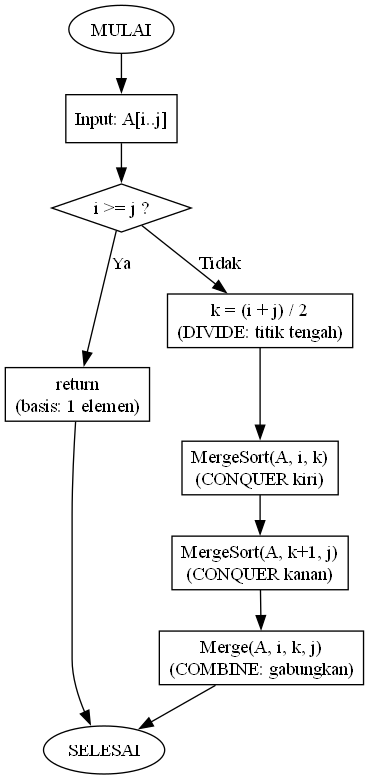
\includegraphics[width=0.45\textwidth]{figures/praktikum4/flowchart_mergesort.png}
    \caption{Flowchart Algoritma Merge Sort}
\end{figure}

\subsubsection*{Flowchart Quick Sort}
\begin{figure}[H]
    \centering
    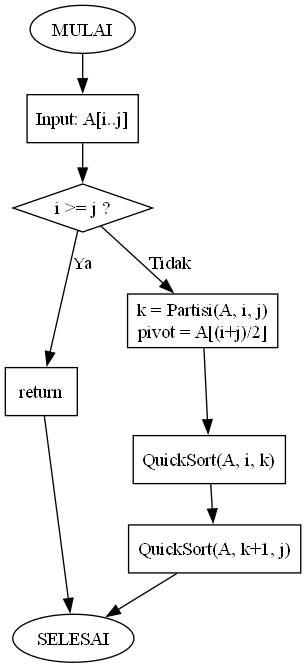
\includegraphics[width=0.45\textwidth]{figures/praktikum4/flowchart_quicksort.png}
    \caption{Flowchart Algoritma Quick Sort}
\end{figure}

\subsubsection*{Source Code Python: MinMaks D\&C}
\begin{lstlisting}[basicstyle=\ttfamily\scriptsize, frame=single, backgroundcolor=\color{white}, numbers=none, keywordstyle=\color{black}, commentstyle=\color{black}, stringstyle=\color{black}, breaklines=true]
def minmaks(arr, i, j):
    # basis: 1 elemen
    if i == j:
        return arr[i], arr[i]
        
    # basis: 2 elemen, bandingkan langsung
    if i == j - 1:
        if arr[i] < arr[j]:
            return arr[i], arr[j]
        else:
            return arr[j], arr[i]
            
    # rekursif: bagi tabel di titik tengah
    k = (i + j) // 2
    min1, maks1 = minmaks(arr, i, k)
    min2, maks2 = minmaks(arr, k + 1, j)
    
    # combine: ambil min dan maks dari kedua bagian
    return min(min1, min2), max(maks1, maks2)
\end{lstlisting}

\subsubsection*{Source Code Python: Merge Sort}
\begin{lstlisting}[basicstyle=\ttfamily\scriptsize, frame=single, backgroundcolor=\color{white}, numbers=none, keywordstyle=\color{black}, commentstyle=\color{black}, stringstyle=\color{black}, breaklines=true]
def merge(arr, kiri, tengah, kanan):
    # salin dua bagian ke array sementara
    kidal1 = arr[kiri:tengah + 1]
    kidal2 = arr[tengah + 1:kanan + 1]
    
    i = j = 0
    k = kiri
    
    # gabungkan dua bagian secara terurut
    while i < len(kidal1) and j < len(kidal2):
        if kidal1[i] <= kidal2[j]:
            arr[k] = kidal1[i]
            i += 1
        else:
            arr[k] = kidal2[j]
            j += 1
        k += 1
        
    # salin sisa elemen kiri jika ada
    while i < len(kidal1):
        arr[k] = kidal1[i]
        i += 1
        k += 1
        
    # salin sisa elemen kanan jika ada
    while j < len(kidal2):
        arr[k] = kidal2[j]
        j += 1
        k += 1

def merge_sort(arr, i, j):
    # basis: array 1 elemen sudah terurut
    if i >= j:
        return
        
    # divide: tentukan titik tengah
    k = (i + j) // 2
    
    # conquer: urutkan bagian kiri dan kanan secara rekursif
    merge_sort(arr, i, k)
    merge_sort(arr, k + 1, j)
    
    # combine: gabungkan hasil pengurutan
    merge(arr, i, k, j)
\end{lstlisting}

\subsubsection*{Source Code Python: Quick Sort}
\begin{lstlisting}[basicstyle=\ttfamily\scriptsize, frame=single, backgroundcolor=\color{white}, numbers=none, keywordstyle=\color{black}, commentstyle=\color{black}, stringstyle=\color{black}, breaklines=true]
def partisi(arr, i, j):
    # pilih elemen tengah sebagai pivot
    pivot = arr[(i + j) // 2]
    p, q = i, j
    
    while True:
        # scan dari kiri sampai menemukan elemen >= pivot
        while arr[p] < pivot:
            p += 1
        # scan dari kanan sampai menemukan elemen <= pivot
        while arr[q] > pivot:
            q -= 1
            
        # jika belum bertemu, tukar dan geser indeks
        if p < q:
            arr[p], arr[q] = arr[q], arr[p]
            p += 1
            q -= 1
        else:
            break
            
    return q

def quick_sort(arr, i, j):
    # basis: array 1 elemen atau kosong
    if i >= j:
        return
        
    # partisi dan dapatkan indeks pembagi
    k = partisi(arr, i, j)
    
    # rekursif urutkan bagian kiri dan kanan
    quick_sort(arr, i, k)
    quick_sort(arr, k + 1, j)

if __name__ == "__main__":
    data = [4, 12, 23, 9, 21, 1, 35, 2, 24]
    print("Data awal:", data)
    
    # MinMaks D&C
    mn, mx = minmaks(data, 0, len(data) - 1)
    print(f"\nMinMaks D&C -> Min: {mn}, Maks: {mx}")
    
    # Merge Sort
    arr_ms = data.copy()
    merge_sort(arr_ms, 0, len(arr_ms) - 1)
    print(f"Merge Sort -> {arr_ms}")
    
    # Quick Sort
    arr_qs = data.copy()
    quick_sort(arr_qs, 0, len(arr_qs) - 1)
    print(f"Quick Sort -> {arr_qs}")
\end{lstlisting}

\subsubsection*{Analisis Output}
Program dijalankan dengan data awal [4, 12, 23, 9, 21, 1, 35, 2, 24]:

\begin{table}[H]
    \centering
    \caption{Output Hasil Pengujian Algoritma Divide and Conquer}
    \begin{tabular}{p{3cm}p{5cm}p{6cm}}
    \toprule
    \textbf{Algoritma} & \textbf{Output} & \textbf{Keterangan} \\ \midrule
    MinMaks D\&C & Min: 1, Maks: 35 & Ditemukan dengan T(n) = O(n) perbandingan \\
    Merge Sort & [1, 2, 4, 9, 12, 21, 23, 24, 35] & Terurut stabil, O(n log n) \\
    Quick Sort & [1, 2, 4, 9, 12, 21, 23, 24, 35] & Terurut, rata-rata O(n log n) \\ \bottomrule
    \end{tabular}
\end{table}

\textbf{MinMaks D\&C:} Tabel dibagi dua pada k=4. Bagian kiri [4,12,23,9,21] menghasilkan min=4, maks=23. Bagian kanan [1,35,2,24] menghasilkan min=1, maks=35. Setelah combine: min=1, maks=35.

\textbf{Merge Sort:} Pembagian berlangsung rekursif hingga setiap bagian berukuran 1 elemen, lalu digabung secara terurut. Karena bersifat stabil, urutan relatif elemen bernilai sama terjaga.

\textbf{Quick Sort:} Pivot dipilih dari elemen tengah setiap iterasi. Proses partisi memindahkan elemen lebih kecil ke kiri dan lebih besar ke kanan pivot, kemudian kedua bagian diurutkan rekursif.

\subsection{Post Test: Merge Sort Standalone}

\subsubsection*{Source Code Python}
\begin{lstlisting}[basicstyle=\ttfamily\scriptsize, frame=single, backgroundcolor=\color{white}, numbers=none, keywordstyle=\color{black}, commentstyle=\color{black}, stringstyle=\color{black}, breaklines=true]
def merge(arr, kiri, tengah, kanan):
    # salin dua bagian ke array sementara
    bagian_kiri = arr[kiri:tengah + 1]
    bagian_kanan = arr[tengah + 1:kanan + 1]
    
    i = j = 0
    k = kiri
    
    # gabungkan dua bagian ke array utama secara terurut
    while i < len(bagian_kiri) and j < len(bagian_kanan):
        if bagian_kiri[i] <= bagian_kanan[j]:
            arr[k] = bagian_kiri[i]
            i += 1
        else:
            arr[k] = bagian_kanan[j]
            j += 1
        k += 1
        
    # salin sisa bagian kiri jika masih ada
    while i < len(bagian_kiri):
        arr[k] = bagian_kiri[i]
        i += 1
        k += 1
        
    # salin sisa bagian kanan jika masih ada
    while j < len(bagian_kanan):
        arr[k] = bagian_kanan[j]
        j += 1
        k += 1

def merge_sort(arr, i, j, depth=0):
    indent = "  " * depth
    # basis: array dengan 1 elemen sudah terurut
    if i >= j:
        return
        
    # divide: hitung titik tengah pembagi
    k = (i + j) // 2
    print(f"{indent}Divide [{i}..{j}] -> kiri [{i}..{k}], kanan [{k+1}..{j}]")
    
    # conquer: urutkan bagian kiri secara rekursif
    merge_sort(arr, i, k, depth + 1)
    
    # conquer: urutkan bagian kanan secara rekursif
    merge_sort(arr, k + 1, j, depth + 1)
    
    # combine: gabungkan hasil pengurutan kedua bagian
    merge(arr, i, k, j)
    print(f"{indent}Combine [{i}..{j}] -> {arr[i:j+1]}")

if __name__ == "__main__":
    data = [38, 27, 43, 3, 9, 82, 10]
    print("Data awal      :", data)
    print("\nProses Merge Sort (D&C):")
    print("-" * 45)
    
    merge_sort(data, 0, len(data) - 1)
    
    print("-" * 45)
    print("Data terurut   :", data)
\end{lstlisting}

\textbf{Jawaban 1: Trace proses Divide-Conquer-Combine}\\
Berikut trace verbose output program dengan data [38, 27, 43, 3, 9, 82, 10]:

\begin{table}[H]
    \centering
    \caption{Trace Eksekusi Merge Sort D\&C}
    \begin{tabular}{cll}
    \toprule
    \textbf{Langkah} & \textbf{Operasi} & \textbf{Hasil} \\ \midrule
    1 & Divide [0..6] -> kiri [0..3], kanan [4..6] & \\
    2 & Divide [0..3] -> kiri [0..1], kanan [2..3] & \\
    3 & Divide [0..1] -> kiri [0..0], kanan [1..1] & \\
    4 & Combine [0..1] & [27, 38] \\
    5 & Divide [2..3] -> kiri [2..2], kanan [3..3] & \\
    6 & Combine [2..3] & [3, 43] \\
    7 & Combine [0..3] & [3, 27, 38, 43] \\
    8 & Divide [4..5] -> kiri [4..4], kanan [5..5] & \\
    9 & Combine [4..5] & [9, 82] \\
    10 & Combine [4..6] & [9, 10, 82] \\
    11 & Combine [0..6] & [3, 9, 10, 27, 38, 43, 82] \\ \bottomrule
    \end{tabular}
\end{table}

\textbf{Jawaban 2: Output eksekusi}\\
Data awal: [38, 27, 43, 3, 9, 82, 10]. Setelah proses Merge Sort D\&C selesai, data terurut menjadi: [3, 9, 10, 27, 38, 43, 82]. Seluruh proses pembagian (Divide) dan penggabungan (Combine) ditampilkan verbose sehingga alur rekursi terlihat jelas dari kedalaman indentasi output.
\subsection{Implementasi Nyata}
Algoritma Merge Sort berbasis Divide and Conquer banyak diimplementasikan pada sistem pengurutan data berskala besar, termasuk pada sistem pemrosesan paralel. Jurnal berikut mendukung relevansi penerapannya.

\vspace{1em}
\textbf{[1] Penulis:} Ketchaya, S. dan Rattanatranurak, A. (2023)

\textbf{Judul:} "Parallel Multi-Deque Partition Dual-Deque Merge Sorting Algorithm Using OpenMP"

\textbf{Publikasi:} Scientific Reports, Vol. 13, Nature Publishing Group. DOI: 10.1038/s41598-023-33583-4

\textbf{Intisari:} Makalah ini mengusulkan algoritma pengurutan paralel berbasis Divide and Conquer yang dikembangkan dari Quick Sort dan Merge Sort menggunakan OpenMP pada sistem memori bersama. Algoritma MPDMSort terbukti lebih efisien dibandingkan implementasi sekuensial standar dalam pengurutan data biologis, saintifik, dan big data. Ini membuktikan bahwa prinsip D\&C yang memecah masalah menjadi upa-masalah independen secara inheren mendukung paralelisme dan skalabilitas.

\textbf{Link:} \url{https://www.ncbi.nlm.nih.gov/pmc/articles/PMC10115789/}

\vspace{1em}
\textbf{Kelebihan dalam konteks nyata:}
\begin{itemize}
    \item Kompleksitas O(n log n) yang konsisten membuat Merge Sort andal untuk pengurutan dataset besar seperti log server, data transaksi, dan rekaman medis.
    \item Sifat stabil Merge Sort menjamin urutan relatif elemen bernilai sama terjaga, penting dalam pengurutan multi-kunci.
    \item Prinsip D\&C secara alami mendukung paralelisasi sehingga cocok untuk sistem multi-core modern.
\end{itemize}

\textbf{Kekurangan dalam konteks nyata:}
\begin{itemize}
    \item Merge Sort membutuhkan memori tambahan O(n) untuk proses penggabungan, sehingga kurang ideal untuk sistem dengan memori terbatas.
    \item Quick Sort memiliki worst case O($n^2$) apabila pemilihan pivot tidak tepat, sehingga perlu strategi pemilihan pivot yang baik seperti median-of-three untuk data dunia nyata.
\end{itemize}
\clearpage

% Praktikum 5
\section{ALGORITMA DECREASE \& CONQUER}
\subsection{Algoritma Decrease and Conquer}
\textbf{Definisi:} Decrease and Conquer adalah metode perancangan algoritma yang mereduksi persoalan berukuran n menjadi beberapa subpersoalan yang lebih kecil, tetapi selanjutnya hanya memproses satu subpersoalan saja secara rekursif. Berbeda dengan Divide and Conquer yang memproses semua subpersoalan dan menggabungkan seluruh solusinya, Decrease and Conquer tidak memiliki tahap combine.

\textbf{Dua Tahap:} 
\begin{enumerate}
    \item \textbf{Decrease:} mereduksi ukuran masalah menjadi subpersoalan yang lebih kecil, biasanya dengan mengurangi satu elemen atau membagi setengah.
    \item \textbf{Conquer:} memproses satu subpersoalan secara rekursif hingga mencapai basis penyelesaian langsung.
\end{enumerate}

\textbf{Tiga Varian:} 
\begin{enumerate}
    \item \textbf{Decrease by a constant:} ukuran masalah berkurang sebesar konstanta tetap setiap iterasi (biasanya 1). Contoh: Selection Sort, Insertion Sort, pencarian sekuensial.
    \item \textbf{Decrease by a constant factor:} ukuran masalah berkurang sebesar faktor tetap setiap iterasi (biasanya 2). Contoh: Binary Search, Fake Coin Problem.
    \item \textbf{Decrease by a variable size:} ukuran pengurangan bervariasi tiap iterasi. Contoh: BST search, Selection Problem.
\end{enumerate}

\textbf{Fungsi:} Digunakan untuk menyelesaikan persoalan yang dapat disederhanakan secara bertahap dengan mereduksi ukuran masalah, seperti pengurutan, pencarian, dan traversal.

\textbf{Kelebihan:} Lebih sederhana dari D\&C karena tidak memerlukan tahap combine, overhead rekursi lebih kecil, dan cocok untuk masalah yang solusinya dapat ditemukan dengan mereduksi satu elemen setiap langkah.

\textbf{Kekurangan:} Tidak seefisien D\&C untuk masalah yang secara alami dapat diparalelkan, dan kompleksitas bisa tetap O($n^2$) apabila strategi pereduksian tidak optimal.

\subsection{Selection Sort sebagai Decrease and Conquer}
Selection Sort adalah contoh klasik varian Decrease by a Constant (k=1). Pada setiap langkah, masalah pengurutan array A[i..j] direduksi menjadi submasalah A[i+1..j] dengan cara meletakkan elemen terkecil di posisi i melalui fungsi Bagi. Tidak ada tahap combine, karena posisi A[i] sudah final setelah fungsi Bagi dijalankan.

Kompleksitas waktu: T(n) = T(n-1) + (n-1) sehingga T(n) = n(n-1)/2 = O($n^2$).
\subsection{Pre Test}
Jawaban pre test praktikum 5.
\subsection{Langkah Praktikum: Selection Sort D\&C}

\subsubsection*{Flowchart}
\begin{figure}[H]
    \centering
    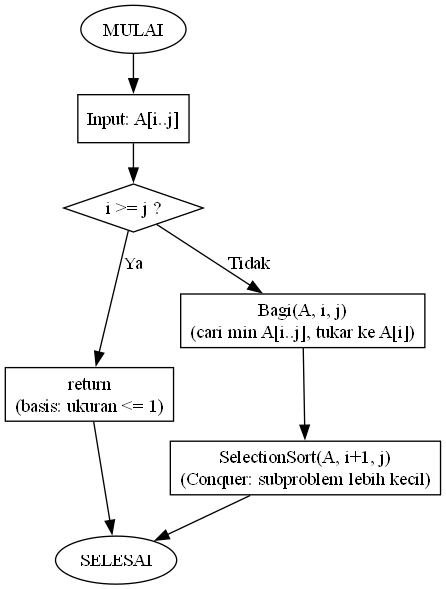
\includegraphics[width=0.45\textwidth]{figures/praktikum5/flowchart_selection_sort_dc.png}
    \caption{Flowchart Algoritma Selection Sort Decrease and Conquer}
\end{figure}

\subsubsection*{Source Code Python}
\begin{lstlisting}[basicstyle=\ttfamily\scriptsize, frame=single, backgroundcolor=\color{white}, numbers=none, keywordstyle=\color{black}, commentstyle=\color{black}, stringstyle=\color{black}, breaklines=true]
def bagi(arr, i, j):
    # cari indeks elemen terkecil dari A[i..j]
    idx_min = i
    for k in range(i + 1, j + 1):
        if arr[k] < arr[idx_min]:
            idx_min = k
            
    # tukar elemen terkecil ke posisi i
    arr[i], arr[idx_min] = arr[idx_min], arr[i]

def selection_sort_dc(arr, i, j):
    # basis: ukuran subarray <= 1, sudah terurut
    if i >= j:
        return
        
    # decrease: letakkan elemen terkecil A[i..j] ke posisi i
    bagi(arr, i, j)
    
    # conquer: urutkan sisa subarray A[i+1..j] secara rekursif
    selection_sort_dc(arr, i + 1, j)

if __name__ == "__main__":
    arr = [64, 25, 12, 22, 11]
    print("Data awal   :", arr)
    
    selection_sort_dc(arr, 0, len(arr) - 1)
    
    print("Data terurut:", arr)
\end{lstlisting}

\subsubsection*{Analisis Output}
Program dijalankan dengan data awal [64, 25, 12, 22, 11] sesuai modul:

\begin{table}[H]
    \centering
    \caption{Trace Rekursi Selection Sort D\&C}
    \begin{tabular}{lllll}
    \toprule
    \textbf{Rekursi ke} & \textbf{Subarray A[i..j]} & \textbf{Elemen Min} & \textbf{Setelah Bagi} & \textbf{Subproblem} \\ \midrule
    1 & A[0..4] = [64,25,12,22,11] & 11 (idx 4) & [11,25,12,22,64] & A[1..4] \\
    2 & A[1..4] = [25,12,22,64] & 12 (idx 2) & [11,12,25,22,64] & A[2..4] \\
    3 & A[2..4] = [25,22,64] & 22 (idx 3) & [11,12,22,25,64] & A[3..4] \\
    4 & A[3..4] = [25,64] & 25 (idx 3) & [11,12,22,25,64] & A[4..4] \\
    5 & A[4..4] = [64] & basis i>=j & tidak ada tukar & selesai \\ \bottomrule
    \end{tabular}
\end{table}

Output akhir: [11, 12, 22, 25, 64]. Setiap rekursi mereduksi submasalah sebesar 1 elemen (decrease by constant = 1). Tidak ada tahap combine karena posisi A[i] sudah final setelah setiap pemanggilan Bagi.

\subsection{Post Test: Selection Sort dengan Input Pengguna}

\subsubsection*{Source Code Python}
\begin{lstlisting}[basicstyle=\ttfamily\scriptsize, frame=single, backgroundcolor=\color{white}, numbers=none, keywordstyle=\color{black}, commentstyle=\color{black}, stringstyle=\color{black}, breaklines=true]
def bagi(arr, i, j):
    # cari indeks elemen terkecil dari A[i..j]
    idx_min = i
    for k in range(i + 1, j + 1):
        if arr[k] < arr[idx_min]:
            idx_min = k
            
    # tukar elemen terkecil ke posisi i
    arr[i], arr[idx_min] = arr[idx_min], arr[i]

def selection_sort_dc(arr, i, j):
    # basis: ukuran subarray <= 1, sudah terurut
    if i >= j:
        return
        
    # decrease: letakkan elemen terkecil ke posisi i
    bagi(arr, i, j)
    
    # conquer: rekursif pada subarray yang lebih kecil
    selection_sort_dc(arr, i + 1, j)

if __name__ == "__main__":
    # terima input array dari pengguna
    raw = input("Masukkan bilangan dipisah spasi: ")
    arr = list(map(int, raw.split()))
    
    print("Data awal   :", arr)
    selection_sort_dc(arr, 0, len(arr) - 1)
    print("Data terurut:", arr)
\end{lstlisting}

\subsubsection*{Analisis Output}
Program menerima input dari pengguna berupa bilangan yang dipisah spasi, mengonversinya ke list integer, lalu menjalankan Selection Sort D\&C. Contoh eksekusi dengan input "5 3 8 1 9 2":

\begin{table}[H]
    \centering
    \caption{Output Hasil Selection Sort Input Pengguna}
    \begin{tabular}{lll}
    \toprule
    \textbf{Input} & \textbf{Data Awal} & \textbf{Data Terurut} \\ \midrule
    5 3 8 1 9 2 & [5, 3, 8, 1, 9, 2] & [1, 2, 3, 5, 8, 9] \\ \bottomrule
    \end{tabular}
\end{table}

Implementasi ini membuktikan bahwa Selection Sort berbasis Decrease and Conquer menghasilkan output yang identik dengan versi iteratif, dengan alur rekursi yang lebih eksplisit mencerminkan prinsip decrease by a constant.
\subsection{Implementasi Nyata}
Pendekatan Decrease and Conquer pada Selection Sort telah dikaji secara akademis untuk penerapan paralel pada sistem komputasi modern. Jurnal berikut mendukung relevansinya.

\vspace{1em}
\textbf{[1] Penulis:} Ganapathi, P. dan Chowdhury, R. (2022)

\textbf{Judul:} "Parallel Divide-and-Conquer Algorithms for Bubble Sort, Selection Sort and Insertion Sort"

\textbf{Publikasi:} The Computer Journal, Vol. 65, No. 10, Hal. 2709-2719. Oxford University Press. DOI: 10.1093/comjnl/bxab107

\textbf{Intisari:} Makalah ini menyajikan algoritma rekursif berbasis Decrease and Conquer untuk Selection Sort, Bubble Sort, dan Insertion Sort yang diparalelkan menggunakan Intel Cilk Plus dengan 32 thread. Hasil eksperimen menunjukkan Selection Sort rekursif D\&C mencapai speedup hingga ratusan kali dibanding versi sekuensialnya pada input terurut terbalik, membuktikan bahwa struktur D\&C secara inheren mendukung paralelisme meskipun kompleksitas asimtotiknya tetap O($n^2$).

\textbf{Link:} \url{https://academic.oup.com/comjnl/article/65/10/2709/6334046}

\vspace{1em}
\textbf{Kelebihan dalam konteks nyata:}
\begin{itemize}
    \item Struktur rekursif Decrease and Conquer secara alami mendukung paralelisasi, memungkinkan speedup signifikan pada sistem multi-core untuk data berukuran sedang.
    \item Implementasi rekursif lebih mudah dibuktikan kebenarannya secara formal dibanding versi iteratif, penting dalam sistem kritis seperti avionik atau medis.
    \item Cocok untuk dataset kecil hingga menengah pada embedded system yang memerlukan algoritma sederhana dengan footprint memori minimal.
\end{itemize}

\textbf{Kekurangan dalam konteks nyata:}
\begin{itemize}
    \item Kompleksitas O($n^2$) tetap tidak berubah meskipun direkursifkan, sehingga tidak disarankan untuk dataset besar dibanding Merge Sort atau Quick Sort.
    \item Overhead pemanggilan fungsi rekursif membutuhkan stack memori tambahan, yang perlu diperhatikan pada sistem dengan memori terbatas.
\end{itemize}
\clearpage

% Praktikum 6
\section{ALGORITMA BFS DAN DFS}
\subsection{Definisi}
Konten definisi praktikum 6.
\subsection*{Pertanyaan 1: Analisis graf berarah pada Gambar 6.4 dan tuliskan urutan jalurnya secara manual apabila menggunakan algoritma BFS dan DFS mulai dari simpul/node ke-0!}

\textbf{Graf Gambar 6.4 (7 simpul):} Edge: 0 $\rightarrow$ 1, 0 $\rightarrow$ 2, 1 $\rightarrow$ 3, 2 $\rightarrow$ 3, 2 $\rightarrow$ 4, 3 $\rightarrow$ 5, 4 $\rightarrow$ 5, 4 $\rightarrow$ 6

\begin{figure}[H]
    \centering
    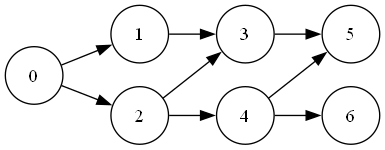
\includegraphics[width=0.65\textwidth]{figures/praktikum6/graf_pretest.png}
    \caption{Visualisasi Graf Pre Test (Gambar 6.4)}
\end{figure}
\vspace{1em}
\textbf{Jawaban BFS manual dari node 0:}
\begin{table}[H]
    \centering
    \caption{Penelusuran BFS Manual dari Node 0}
    \begin{tabular}{lllp{6cm}}
    \toprule
    \textbf{Langkah} & \textbf{Node Diproses} & \textbf{Antrian Setelah} & \textbf{Alasan} \\ \midrule
    1 & 0 & [1, 2] & kunjungi 0, masukkan tetangga 1 dan 2 \\
    2 & 1 & [2, 3] & kunjungi 1, masukkan tetangga 3 \\
    3 & 2 & [3, 4] & kunjungi 2, masukkan 4 (3 sudah di antrian) \\
    4 & 3 & [4, 5] & kunjungi 3, masukkan tetangga 5 \\
    5 & 4 & [5, 6] & kunjungi 4, masukkan 6 (5 sudah di antrian) \\
    6 & 5 & [6] & kunjungi 5, tidak ada tetangga baru \\
    7 & 6 & [] & kunjungi 6, tidak ada tetangga baru \\ \bottomrule
    \end{tabular}
\end{table}
Urutan BFS: 0, 1, 2, 3, 4, 5, 6

\vspace{1em}
\textbf{Jawaban DFS manual dari node 0:}
\begin{table}[H]
    \centering
    \caption{Penelusuran DFS Manual dari Node 0}
    \begin{tabular}{llp{9cm}}
    \toprule
    \textbf{Langkah} & \textbf{Node} & \textbf{Aksi} \\ \midrule
    1 & 0 & kunjungi 0, rekursi ke tetangga pertama: 1 \\
    2 & 1 & kunjungi 1, rekursi ke tetangga: 3 \\
    3 & 3 & kunjungi 3, rekursi ke tetangga: 5 \\
    4 & 5 & kunjungi 5, tidak ada tetangga, backtrack ke 3, ke 1, ke 0 \\
    5 & 2 & dari 0 rekursi ke tetangga berikutnya: 2 \\
    6 & 4 & kunjungi 2, rekursi ke 4 (3 dan 5 sudah dikunjungi) \\
    7 & 6 & kunjungi 4, rekursi ke 6 (5 sudah dikunjungi) \\ \bottomrule
    \end{tabular}
\end{table}
Urutan DFS: 0, 1, 3, 5, 2, 4, 6

\subsection*{Pertanyaan 2: Apa perbedaan utama antara algoritma BFS dan DFS?}

\begin{table}[H]
    \centering
    \caption{Perbedaan Algoritma BFS dan DFS}
    \begin{tabular}{p{3.5cm}p{5cm}p{5cm}}
    \toprule
    \textbf{Aspek} & \textbf{BFS} & \textbf{DFS} \\ \midrule
    Strategi penelusuran & Melebar (level by level) & Mendalam (cabang habis dulu) \\
    Struktur data & Queue (antrian) & Stack / Rekursi \\
    Kompleksitas memori & O(V) untuk antrian & O(H), H = kedalaman rekursi \\
    Jalur terpendek & Menjamin pada graf tidak berbobot & Tidak menjamin \\
    Penggunaan utama & Shortest path, web crawling & Deteksi siklus, topological sort \\
    Kompleksitas waktu & O(V + E) & O(V + E) \\ \bottomrule
    \end{tabular}
\end{table}
\subsection{Langkah Praktikum: BFS dan DFS pada Graf 6.1}

\begin{figure}[H]
    \centering
    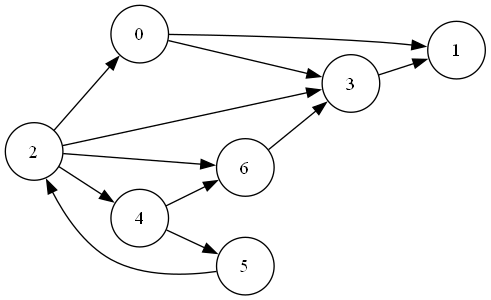
\includegraphics[width=0.65\textwidth]{figures/praktikum6/graf_praktikum.png}
    \caption{Visualisasi Graf Berarah Gambar 6.1 (Langkah Praktikum)}
\end{figure}

\subsubsection*{Flowchart BFS}
\begin{figure}[H]
    \centering
    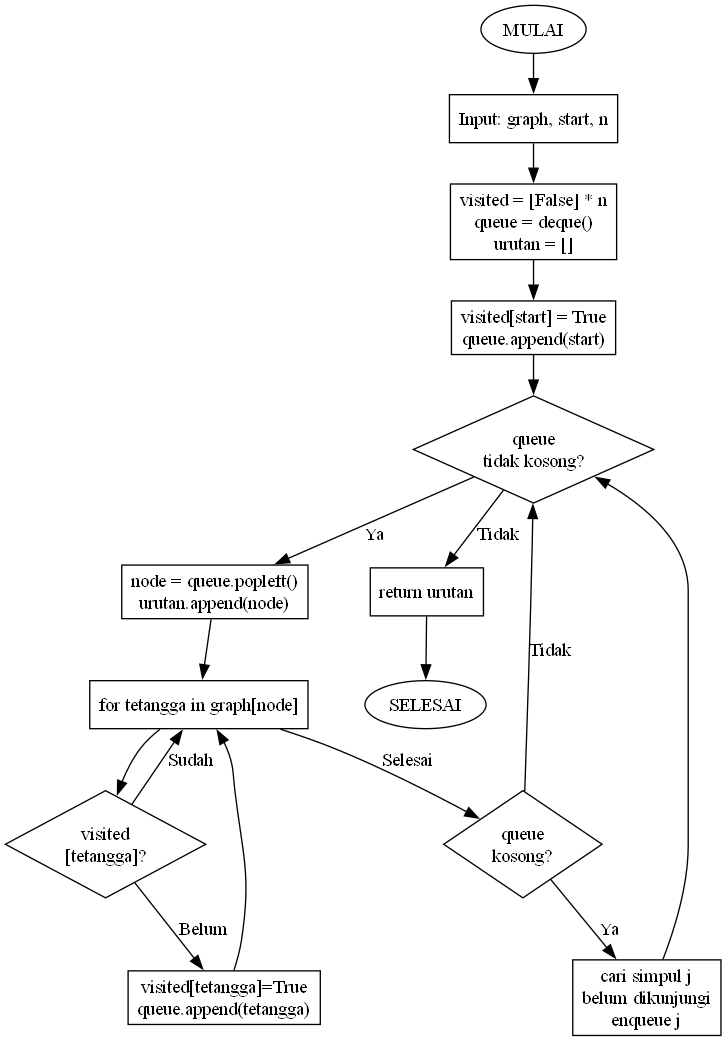
\includegraphics[width=0.45\textwidth]{figures/praktikum6/flowchart_bfs.png}
    \caption{Flowchart Algoritma BFS}
\end{figure}

\subsubsection*{Flowchart DFS}
\begin{figure}[H]
    \centering
    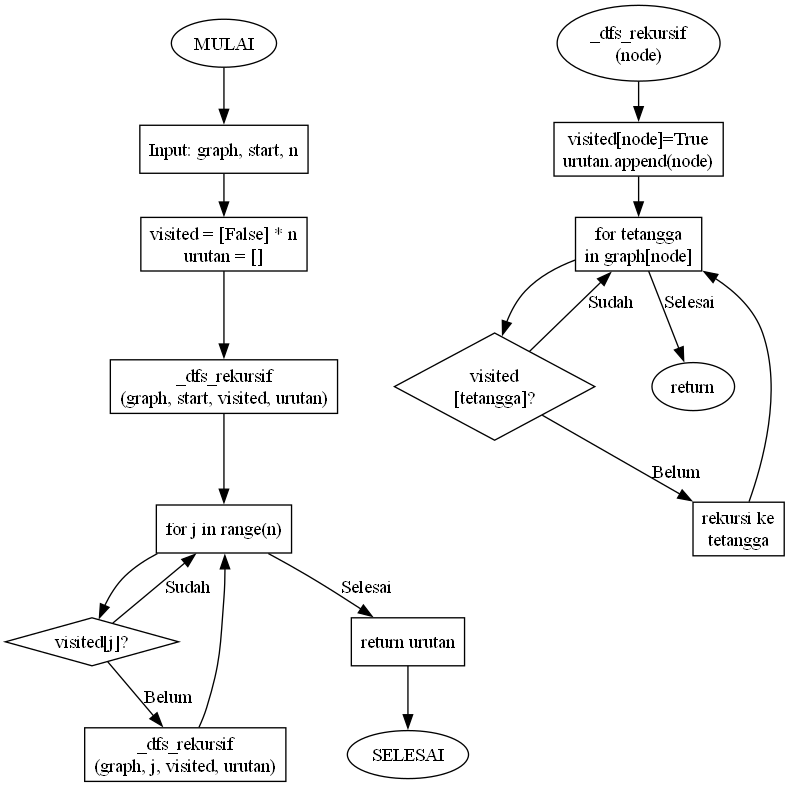
\includegraphics[width=0.45\textwidth]{figures/praktikum6/flowchart_dfs.png}
    \caption{Flowchart Algoritma DFS}
\end{figure}

\subsubsection*{Source Code Python: BFS}
\begin{lstlisting}[basicstyle=\ttfamily\scriptsize, frame=single, backgroundcolor=\color{white}, numbers=none, keywordstyle=\color{black}, commentstyle=\color{black}, stringstyle=\color{black}, breaklines=true]
def bfs(graph, start, n):
    visited = [False] * n
    urutan = []
    queue = deque()
    
    # tandai simpul awal sebagai dikunjungi dan masukkan ke antrian
    visited[start] = True
    queue.append(start)
    
    while queue:
        # ambil simpul paling depan antrian
        node = queue.popleft()
        urutan.append(node)
        
        # kunjungi semua tetangga yang belum dikunjungi
        for tetangga in graph[node]:
            if not visited[tetangga]:
                visited[tetangga] = True
                queue.append(tetangga)
                
        # jika antrian kosong tapi masih ada simpul yang belum dikunjungi
        if not queue:
            for j in range(n):
                if not visited[j]:
                    visited[j] = True
                    queue.append(j)
                    break
                    
    return urutan

if __name__ == "__main__":
    # graf berarah Gambar 6.1 sesuai kode tester modul
    n = 7
    graph = {
        0: [1, 3],
        1: [],
        2: [0, 3, 4, 6],
        3: [1],
        4: [5, 6],
        5: [2],
        6: [3],
    }
    hasil = bfs(graph, 0, n)
    print("BFS mulai dari node 0:", hasil)
\end{lstlisting}

\subsubsection*{Source Code Python: DFS}
\begin{lstlisting}[basicstyle=\ttfamily\scriptsize, frame=single, backgroundcolor=\color{white}, numbers=none, keywordstyle=\color{black}, commentstyle=\color{black}, stringstyle=\color{black}, breaklines=true]
def _dfs_rekursif(graph, node, visited, urutan):
    # tandai simpul saat ini sebagai dikunjungi
    visited[node] = True
    urutan.append(node)
    
    # kunjungi semua tetangga yang belum dikunjungi secara rekursif
    for tetangga in graph[node]:
        if not visited[tetangga]:
            _dfs_rekursif(graph, tetangga, visited, urutan)

def dfs(graph, start, n):
    visited = [False] * n
    urutan = []
    
    # mulai DFS dari simpul awal
    _dfs_rekursif(graph, start, visited, urutan)
    
    # tangani simpul yang belum terjangkau
    for j in range(n):
        if not visited[j]:
            _dfs_rekursif(graph, j, visited, urutan)
            
    return urutan

if __name__ == "__main__":
    # graf berarah Gambar 6.1 sesuai kode tester modul
    n = 7
    graph = {
        0: [1, 3],
        1: [],
        2: [0, 3, 4, 6],
        3: [1],
        4: [5, 6],
        5: [2],
        6: [3],
    }
    hasil = dfs(graph, 0, n)
    print("DFS mulai dari node 0:", hasil)
\end{lstlisting}

\subsubsection*{Analisis Output dan Perbedaan Kedua Algoritma}
Program dijalankan pada graf berarah Gambar 6.1 (7 simpul) dimulai dari node 0. Graf memiliki edge: 0$\rightarrow$1, 0$\rightarrow$3, 2$\rightarrow$0, 2$\rightarrow$3, 2$\rightarrow$4, 2$\rightarrow$6, 3$\rightarrow$1, 4$\rightarrow$5, 4$\rightarrow$6, 5$\rightarrow$2, 6$\rightarrow$3.

\begin{table}[H]
    \centering
    \caption{Perbandingan Urutan Traversal BFS dan DFS}
    \begin{tabular}{llp{3cm}p{3cm}}
    \toprule
    \textbf{Algoritma} & \textbf{Urutan Traversal} & \textbf{Simpul ke-5 dikunjungi ke-} & \textbf{Simpul ke-6 dikunjungi ke-} \\ \midrule
    BFS & [0, 1, 3, 2, 4, 6, 5] & ke-7 (terakhir) & ke-6 \\
    DFS & [0, 1, 3, 2, 4, 5, 6] & ke-6 & ke-7 (terakhir) \\ \bottomrule
    \end{tabular}
\end{table}

Perbedaan terlihat pada urutan kunjungan simpul 5 dan 6. BFS mengunjungi simpul 6 sebelum 5 karena 6 masuk antrian lebih dulu (saat memproses simpul 4, edge 4$\rightarrow$6 diperiksa sebelum 4$\rightarrow$5 jika indeks lebih kecil diutamakan). DFS sebaliknya, masuk ke simpul 5 terlebih dahulu mengikuti cabang 4$\rightarrow$5 sebelum backtrack ke 4$\rightarrow$6.

\subsubsection*{Visualisasi Urutan Traversal}

\begin{figure}[H]
    \centering
    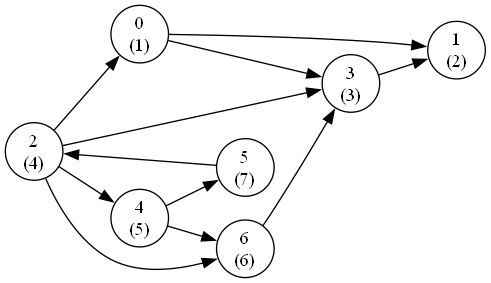
\includegraphics[width=0.65\textwidth]{figures/praktikum6/graf_bfs.png}
    \caption{Urutan BFS dari Node 0 (angka dalam kurung = urutan kunjungan)}
\end{figure}

\begin{figure}[H]
    \centering
    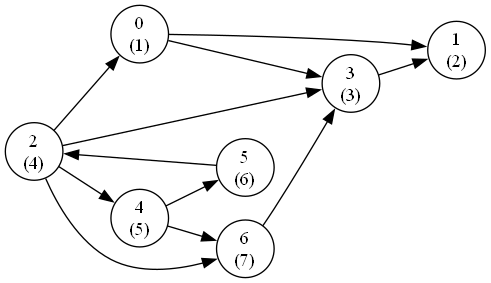
\includegraphics[width=0.65\textwidth]{figures/praktikum6/graf_dfs.png}
    \caption{Urutan DFS dari Node 0 (angka dalam kurung = urutan kunjungan)}
\end{figure}

\subsection{Post Test: BFS dan DFS pada Graf Pre Test (Gambar 6.4)}

\subsubsection*{Source Code Python}
\begin{lstlisting}[basicstyle=\ttfamily\scriptsize, frame=single, backgroundcolor=\color{white}, numbers=none, keywordstyle=\color{black}, commentstyle=\color{black}, stringstyle=\color{black}, breaklines=true]
from collections import deque

def bfs(graph, start, n):
    visited = [False] * n
    urutan = []
    queue = deque()
    
    # tandai simpul awal dan masukkan ke antrian
    visited[start] = True
    queue.append(start)
    
    while queue:
        node = queue.popleft()
        urutan.append(node)
        
        # kunjungi tetangga yang belum dikunjungi
        for tetangga in graph[node]:
            if not visited[tetangga]:
                visited[tetangga] = True
                queue.append(tetangga)
                
        # tangani simpul tidak terjangkau
        if not queue:
            for j in range(n):
                if not visited[j]:
                    visited[j] = True
                    queue.append(j)
                    break
                    
    return urutan

def _dfs_rekursif(graph, node, visited, urutan):
    # tandai dan catat simpul yang dikunjungi
    visited[node] = True
    urutan.append(node)
    
    # rekursif ke tetangga yang belum dikunjungi
    for tetangga in graph[node]:
        if not visited[tetangga]:
            _dfs_rekursif(graph, tetangga, visited, urutan)

def dfs(graph, start, n):
    visited = [False] * n
    urutan = []
    
    _dfs_rekursif(graph, start, visited, urutan)
    
    # tangani simpul yang belum terjangkau
    for j in range(n):
        if not visited[j]:
            _dfs_rekursif(graph, j, visited, urutan)
            
    return urutan
\end{lstlisting}

\textbf{Jawaban 1: Penerapan BFS dan DFS pada graf Gambar 6.4}\\
Program dijalankan pada graf pre test (Gambar 6.4) dengan 7 simpul mulai dari node 0:

\begin{table}[H]
    \centering
    \caption{Validasi Hasil Program vs Manual pada Graf Pre Test}
    \begin{tabular}{lllp{1.5cm}}
    \toprule
    \textbf{Algoritma} & \textbf{Hasil Program} & \textbf{Jawaban Manual Pre Test} & \textbf{Sama?} \\ \midrule
    BFS & [0, 1, 2, 3, 4, 5, 6] & [0, 1, 2, 3, 4, 5, 6] & Ya \\
    DFS & [0, 1, 3, 5, 2, 4, 6] & [0, 1, 3, 5, 2, 4, 6] & Ya \\ \bottomrule
    \end{tabular}
\end{table}

\textbf{Jawaban 2: Analisis kesesuaian hasil program dengan jawaban pre test}\\
Hasil program sepenuhnya sesuai dengan jawaban manual pre test untuk kedua algoritma. Ini memvalidasi bahwa:
\begin{enumerate}
    \item Implementasi Python BFS menggunakan \texttt{deque} sudah benar dalam mengeksplorasi graf secara berlapis, menghasilkan urutan yang identik dengan penelusuran manual menggunakan antrian.
    \item Implementasi Python DFS rekursif sudah benar dalam mengeksplorasi graf secara mendalam, menghasilkan urutan yang identik dengan penelusuran manual menggunakan prinsip backtracking.
    \item Penanganan simpul tidak terjangkau (isolated nodes) sudah ditangani dengan benar di kedua implementasi sehingga seluruh 7 simpul berhasil dikunjungi.
\end{enumerate}
\subsection{Implementasi Nyata}
Algoritma BFS dan DFS merupakan fondasi dari banyak aplikasi dunia nyata mulai dari navigasi, jaringan sosial, hingga analisis jaringan komputer. Jurnal berikut mendukung relevansinya.

\vspace{1em}
\textbf{[1] Penulis:} Ahmed, R., Chekol, B., dan Alsaleh, M. (2025)

\textbf{Judul:} "HDBMS: A Context-Aware Hybrid Graph Traversal Algorithm for Efficient Information Discovery in Social Networks"

\textbf{Publikasi:} arXiv preprint arXiv:2508.14092, Uskudar University, Istanbul, 2025.

\textbf{Intisari:} Makalah ini mengusulkan algoritma traversal hibrid berbasis BFS dan DFS yang dinamis dan adaptif untuk jaringan sosial. Eksperimen pada berbagai graf berarah menunjukkan bahwa BFS unggul dalam menemukan jalur terpendek antar pengguna (misal pencarian teman terdekat), sedangkan DFS lebih efisien dalam menelusuri rantai hubungan yang dalam (misal rantai influencer). Karya ini menegaskan bahwa pemilihan algoritma traversal harus disesuaikan dengan konteks dan struktur graf yang dihadapi.

\textbf{Link:} \url{https://arxiv.org/pdf/2508.14092}

\vspace{1em}
\textbf{Kelebihan dalam konteks nyata:}
\begin{itemize}
    \item BFS unggul untuk pencarian jalur terpendek pada jaringan tidak berbobot seperti jaringan sosial (degree of separation), routing paket jaringan, dan rekomendasi koneksi.
    \item DFS unggul untuk eksplorasi mendalam seperti deteksi siklus dalam dependency graph, topological sort pada build system, dan traversal struktur file sistem operasi.
    \item Kompleksitas O(V+E) yang sama membuat keduanya efisien untuk graf skala menengah dan dapat dioptimalkan lebih lanjut dengan teknik paralel untuk graf berskala besar.
\end{itemize}

\textbf{Kekurangan dalam konteks nyata:}
\begin{itemize}
    \item BFS membutuhkan memori besar O(V) untuk antrian, tidak cocok untuk graf dengan jutaan simpul seperti graf internet tanpa optimasi memori.
    \item DFS berisiko stack overflow pada graf sangat dalam apabila diimplementasikan secara rekursif, dan perlu diubah ke iteratif berbasis stack eksplisit untuk sistem produksi.
\end{itemize}
\clearpage

% DAFTAR PUSTAKA
\phantomsection
\addcontentsline{toc}{section}{DAFTAR PUSTAKA}
\nocite{*}
\printbibliography[title={DAFTAR PUSTAKA}]
\clearpage

\end{document}